\section{Methods}\label{sec:methods}

\asubsection{Layers}{Maria Stickel}\label{sec:layers}

In the following we'll describe the different layers we implemented. We define $\mathcal{LL}$(\texttt{Layer}) to be the log-likelihood contribution of \texttt{Layer}. We refrain from deducing the formulas for bound looseness and likelihood contribution and refer the reader to \cite{nielsen2020survae}.

All of the layers are defined in the inference direction, i.e. the `forward' method sends elements of the data space $\mathcal{X}$ to the latent space $\mathcal{Z}$, whereas the `backward' method goes from $\mathcal{Z}$ to $\mathcal{X}$.

The layers can be separated in two groups: stochastic and non-stochastic\footnote{In \cite{nielsen2020survae} they refer to the non-stochastic layers as bijective. This was a little confusing in the beginning as some stochastic layers are (in theory) bijective operations on the data (permutations) but also stochastic in the sense that they operate differently in different execution calls on the \textbf{same} data.}. The forward call implements the mapping $\mathcal{X} \rightarrow \mathcal{Z}$. All of our layers are vectorized over the batch size. 


\asubsubsection{\texttt{BijectiveLayer}}{Maria Stickel}\label{sec:bijective}
Standard bijective transformation from normalizing flow architecture. In the forward pass, the input vector is divided into two parts: On the skip part no transformations are applied, but the input is simply passed on as it is. Yet, it serves for the calculation of the bijective non-identity transformation applied to the other part of the data.

Firstly, the skipped input is fed to a standard feed-forward neural network which generates the coefficients $(s,t)$ of the linear transformation applied to the non-skip part. The backward pass (or generative direction) is the inverse transformation. The likelihood contribution of a bijective (non-stochastic) transformation is $ \log | \det (J)|$ where $J$ is the Jacobian of the transformation which in the case of our chosen linear transformation \eqref{eq:bijective} results in a log-likelihood contribution of \eqref{eq:ll_bijective}. 
\begin{equation}
\texttt{ BijectiveLayer} (X_i) = \left\{ \begin{array}{rl}X_i & \text{for $i$ in skip connection} \\ e^{\tanh(s_i)} \cdot X_i + t_i & \text{for $i$ in non-skip connection} \end{array} \right.
\label{eq:bijective}
\end{equation}
\begin{equation}
    \mathcal{LL}\texttt{(BijectiveLayer)}= \sum_{i} \tanh(s_i)
    \label{eq:ll_bijective}
\end{equation}
In the case of labelled input, the bijective layer applies the same transformation, except for the skip-connection, that is extended by the labels. We had quite some issues with this layer in the context of the Point Cloud data described in section \ref{sec:spatial_mnist}. The first version of the layer was structured in a way that it accepted a flattened input vector representing one "point of data" and applied its transformation to it. So we modified it to accept tuples of shape, that we flatten (in the final version of the implementation). The purpose and functionality of the layer is the same as before. The layer applies the bijective transformation to the last \texttt{skip\textunderscore size} points in the point cloud.

\asubsubsection{\texttt{OrthonormalLayer}}{Maria Stickel}\label{sec:orthonormal}
Applies orthonormal transformation and its inverse. Unlike other layers, the transformation is randomly sampled upon initialization and applied every time the network is called (i.e. no training). The likelihood contribution is obviously zero as the determinant of the Jacobian of an orthonormal transformation is one. It is obviously a bijective module. In the case of spatial MNIST, we used a more specific version of this layer (transposition layer), which we did not implement as a separate layer, which swaps the x- and y-components.

\asubsubsection{\texttt{MaxTheLayer}}{Maria Stickel}
The forward pass consists of taking the maximum over the entire input, while the backward pass samples an index $k$ for the maximum value based on a categorical distribution (whose weights can be learned in training) and subtracts values sampled from the half-normal distribution from the maximum value in all other entries. Its variance $\sigma$ can and should be learned and is initially set to $0.1$. The layer is clearly stochastic and therefore has a non-trivial contribution to the log-likelihood approximated in the following way\footnote{A deduction of this can be found in \cite{nielsen2020survae}, more specifically in Appendix E.}.
\begin{equation}
\mathcal{LL}(\texttt{MaxTheLayer}) \approx
   \sum_{i = k} \log p(\text{i}|Z) + \sum_{i \neq k} \log q(X_i|Z,k) 
\end{equation}

\asubsubsection{\texttt{MaxPoolingLayer} \& \texttt{MaxPoolingLayerWithOverlap}}{Maria Stickel}\label{sec:max_pooling_layer}
We implemented a surjective layer with stochastic backward pass that reduces 2-dimensional input data by taking the local maximum over blocks of it. Note that, as mentioned above, the input is generally flattened, so the layer un-flattens the given input\footnote{Which requires flattened-data-shape to be a square nummber.} and then performs the MaxPooling operation. The \texttt{MaxPoolingLayer} has no overlap between blocks, any entry is used for calculation of exactly one local maximum, equal to the layer in \cite{nielsen2020survae}.

In the generative direction of \texttt{MaxPoolingLayer} (the backward pass), the maximum is arbitrarily assigned to one position in the corresponding block and all other block entries are sampled as smaller values by subtracting values sampled by a half-normal (default) or an exponential distribution (choice upon layer definition) from the block maximum (see Table~\ref{table:maxpool_distributions}). Therefore, the log-likelihood contribution is essentially the same as that of \texttt{MaxTheLayer}, just repeated for each block. Distribution parameters are parameters that can be trained (design choice). We recommend to use the option to train them. At this point it is worth mentioning that one could have further extended the flexibility of the layer by training a classifier to assign the argmax value in a block. Another reasonable extension of functionality would be to use several distributions for sampling the values-to-be-subtracted for the \texttt{MaxPoolingLayer}, with different possible parameters i.e. one per block, or one per several blocks, to further adapt to the distribution of the underlying data. These different granularities are a hyperparameter, which we chose to set to one, considering the scope of the project.
\begin{table}[H]
    \centering
    \begin{tabular}{lcc}
    \toprule
    & Half-Normal & Exponential \\
    \midrule
    Formula & $f(x; \sigma) = \sqrt{\frac{2}{\pi}} \frac{1}{\sigma} e^{-\frac{x^2}{2\sigma^2}}$ & $f(x; \lambda) = \lambda e^{-\lambda x}$ \\
    Parameters & $\sigma > 0$ & $\lambda > 0$ \\
    \bottomrule
    \end{tabular}
    \caption{The two distributions that we implemented for \texttt{MaxPoolingLayer} and \texttt{MaxPoolingLayerWithOverlap}.}
    \label{table:maxpool_distributions}
\end{table}
We extended the functionalities in \cite{nielsen2020survae} by implementing a \texttt{MaxPoolingLayerWithOverlap} which is similar, but allows for overlap between the blocks over which the maximum is taken. Figure \ref{fig:both_maxpoolings} illustrates \texttt{MaxPoolingLayerWithOverlap} for different hop sizes, where the stride indicates the block size, the hop is the offset from one block to the next and the width is the width of the picture/data. Strictly speaking, \texttt{MaxPoolingLayer} is a special case of \texttt{MaxPoolingLayerWithOverlap} with stride=hop. For simplicity all input data is assumed to be square.
\begin{figure}
    \centering
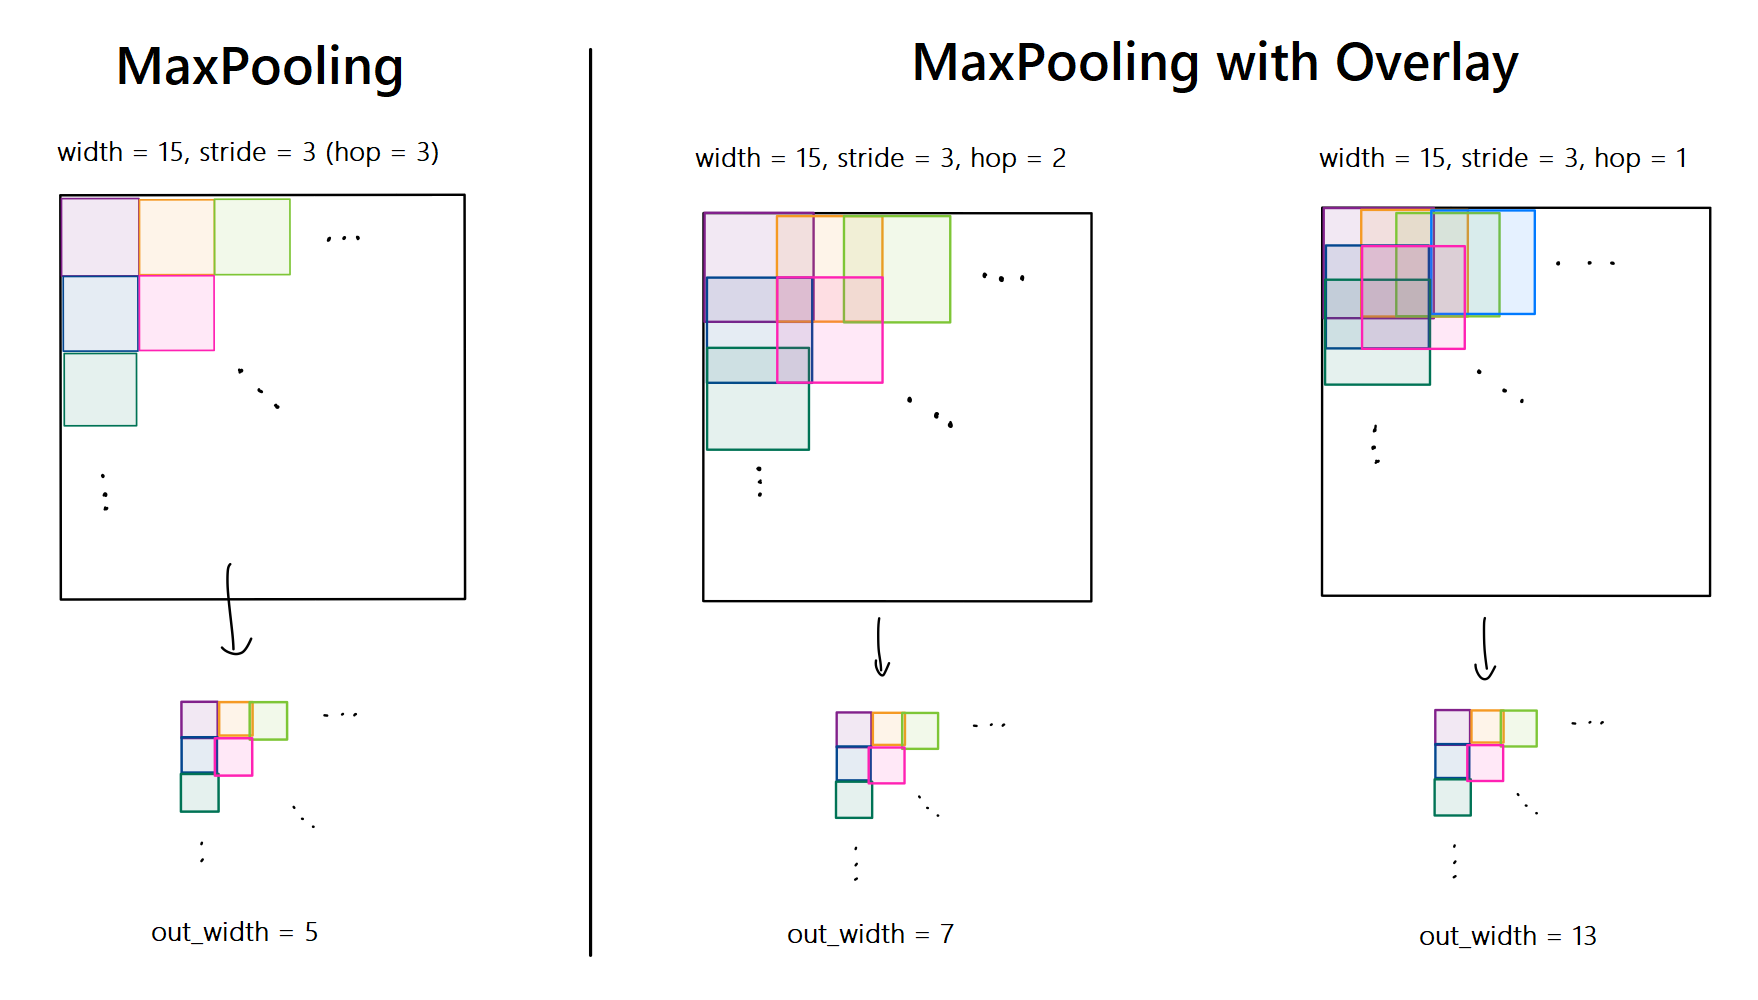
\includegraphics[width=\textwidth]{images/layers/BothMaxPoolings.png}
    \caption{Different parameters for \texttt{MaxPoolingLayerWithOverlap}. The smaller the hop, the larger the output size.}\label{fig:both_maxpoolings}
\end{figure}

The backward pass of \texttt{MaxPoolingLayerWithOverlap} requires a different approach, as the overlap between blocks poses several constraints on an entry, as it needs to be smaller or equal to the smallest maximum of all blocks containing it. We calculate the smallest such maximum for each entry and then sample an index for our maximum in the fields where it actually can be assumed (data-dependent), while subtracting values sampled from a half-normal or an exponential distribution (design choice) with learned parameters.

Similarly to the version of the layer without the overlap, one could think about learning several half-normal or exponential distributions for values to be subtracted. Yet, using a classifier to sample a random index to place the maximum proves to be much more difficult, as candidate amount and location changes depending on the data. We constrained our use cases to square 2D data and used square blocks, but more complex data and block shapes could be used. The approximation of the log-likelihood is similar to the one in \texttt{MaxTheLayer}, only that it's a little bit more complex in practice to perform the computation for all the different blocks.

\asubsubsection{\texttt{SortingLayer}}{Maria Stickel}\label{sec:sorting_layer}
In the forward pass, this layer performs a sorting operation along the last axis. Use cases can be naturally sorted data, exchangeable models and order statistics. It is a stochastic surjective transformation, as we cannot recover the original order of the vector. The backward pass is a random permutation.

We implemented a helper function both for \texttt{SortingLayer} and \texttt{PermutationLayer}, to enable a vectorized treatment of the batch. It applies a random permutation to the last axis of X for each entry along its first axis, and is used in the backward pass of the Sorting Layer. There is a possibility to replace the random permutation in the backwards pass with a categorical distribution with learned parameters, which we did not pursue, making the log-likelihood of this operation zero.


\asubsubsection{\texttt{PermutationLayer}}{Maria Stickel}\label{sec:permutation_layer}
This layer randomly shuffles in both the inference and the generative direction, with a new permutation in each call. This is a stochastic operation with zero contribution to the log-likelihood. Is is used in each block for the Point Cloud data (section \ref{sec:spatial_mnist}) to enforce permutation invariance. 


\asubsubsection{\texttt{AbsoluteLayer}}{Maria Stickel}\label{sec:absolute_layer}
This layer performs the absolute value inference surjection. The forward pass is simply taking the absolute value of each entry abs$(X)$. In the backward pass, we sample signs $S$ for all the values in $Z$, using a parameter $q$ (which can be trained or set to a fixed value like $\frac{1}{2}$), which is the event probability of sampling a positive sign, and then return the product of the signs with the data $\hat{X} = S \cdot Z$. The log-likelihood contribution is described in \eqref{eq:ll_absolute} and corresponds to the log-likelihood contribution derived in \cite{nielsen2020survae}, except for the fact that they describe it for one-dimensional input while we extend it to higher-dimensional input (summation). 
\begin{equation}
\mathcal{LL}\text{(\texttt{AbsoluteLayer})} = \#\{S_i : S_i = 1\} \cdot \log(q) +  \#\{S_i : S_i = -1\} \cdot \log(1 - q)  \label{eq:ll_absolute}
\end{equation}
We experimented with different values for $q$, which in theory is supposed to be in $[0,1]$. As it is a trained parameter, it can escape those reasonable bounds. Read more about this in section \ref{sec:exp_and_results}.


\asubsubsection{\texttt{DequantizationLayer}}{Maria Stickel}\label{sec:dequantization_layer}
This layer's purpose is to un-discretize, which is adding random noise in $(0,1)$ in the forward pass to quantized input data\footnote{Or in programming terms: convert from integer to double (or float).}. This is necessary as we want to be able to generate discrete data while sampling from a Gaussian, which requires de-quantization in the forward pass. The backward pass is a rounding operation (floor). The log-likelihood of this operation is zero as we use a uniform distribution over the noise interval. We used it for image data, see section \ref{sec:image_data}.


\asubsubsection{\texttt{AugmentLayer}}{Maria Stickel}
As the name suggests, we augment input data by extending data points with randomly sampled values in the forward pass and removing them in the backward pass. In our implementation, we don't learn distribution parameters, but only sample from a standard normal distribution. Therefore in our case the log-likelihood contribution is zero. If given more time, we could have implemented different distributions with their respective (trainable) parameters. The layer has proven to be useful in datasets based on discontiguous distributions (e.g. the two moons dataset). It is surjective in the generative direction.


\asubsubsection{\texttt{SliceLayer}}{Maria Stickel}
This layer is the opposite of \texttt{AugmentLayer}. In the forward pass, we remove elements from the input vector and in the backward pass we augment it. The log-likelihood contribution is zero for the same reason.

\asubsubsection{\texttt{PermuteAxesLayer}}{Maria Stickel}\label{sec:permute_axes_layer}
As the name suggests, this layer permutes the axes of the vector space. Obviously, this is only useful for multi-dimensional data and is used in particular for the Point Cloud Data.


\asubsubsection{\texttt{ReshapeLayer}}{Maria Stickel}\label{sec:reshape_layer}
A layer to reshape data vectors. We implemented it for the spatial MNIST dataset, to reshape the output to point cloud elements.

\asubsection{Training}{Tomáš Sláma}

The training of all models was done via the Adam optimizer in batches of size $k$, meaning each of the $n$ epochs sampled $k$ values $X$ from the dataset function.
It then ran $X$ forward through the network, obtaining the values in latent space $Z$, along with the log-likelihood $\mathcal{LL}$, and ran a step of the optimizer on their sum; more specifically: $$\mathcal{L}\text{oss} = 0.5 |Z|^2 - \mathcal{LL}$$
The training also supports decaying the learning rate (which was used for most of the examples) and providing the layers with conditional vector, which was used for training conditional networks (by influencing how the log-likelihood was calculated).

Besides returning the trained network, the training function also saved state snapshots and losses on an evaluation set to prevent overfitting in an orderly way, making plotting easy. 

\asubsection{Model Evaluation}{Jannis Heising}

Since the two-dimensional synthetic distributions (Section~\ref{sec:synthetic}) are easy to visualize, our main evaluation tool was our own judgment of the distribution plots. Additionally, we always plotted the training and validation losses. Where appropriate, we sought to visualize the behaviour of the novel models from~\cite{nielsen2020survae} in the form of ``Q-plots" (Figure~\ref{fig:skewed-q}) and symmetry axes (Figure~\ref{fig:symmetries_checkerboard}) for the \texttt{AbsoluteLayer}.

For the higher-dimensional datasets, we visualized the code distribution of the trained models by taking the output {$Z = f(X)$} of a model $f$ from a data sample $X$ and plotted one-dimensional and two-dimensional slices of $Z$ (see for example Figure~\ref{fig:spatial_mnist_code_after}). The 1D slices are overlaid with the probability density function of the standard Normal distribution $\mathcal{N}(0, 1)$ and the 2D slices show its 90\% confidence interval for an intuitive visual cue of how well the distributions match (both in red).

Additionally, we used calibration diagrams to gauge how well the samples from a given model fit the observed data distribution (see Figure~\ref{fig:sir_run_1}). Without going into detail, a calibration diagram shows in which ``parts" of the data distribution a given sample (or set of samples) is likely to fall. Ideally, all bars have the same height, indicated by a red dotted line. We ended up only using this tool for the SBI data (Section~\ref{sec:sbi}) because it is fairly low-dimensional but could have theoretically used it for all other tests as well.

The SBI models additionally provided the option to use resimulation diagrams (see Figure~\ref{fig:sir_run_2}): Given an initial set of parameters $X$, one takes the corresponding simulation data $Y$ and generates samples {$\hat{X} = f^{-1}(Z|Y)$} from a trained model $f$. These samples are fed to the simulation to obtain simulation data $\hat{Y}$. One can then determine whether the original data $Y$ lies within the 90\% confidence interval of the new data $\hat{Y}$ by plotting them together.

While trying to find the error in the \texttt{BijectiveLayer} log-likelihood contribution described in Section~\ref{sec:image_data}, we additionally started logging the standard deviation of the code distribution. It turned out that it behaved very similarly to the loss (see Figure~\ref{fig:mnist_run_4_loss_vs_sigma}), so we chose not to mention it except here.

\begin{figure}
\centering
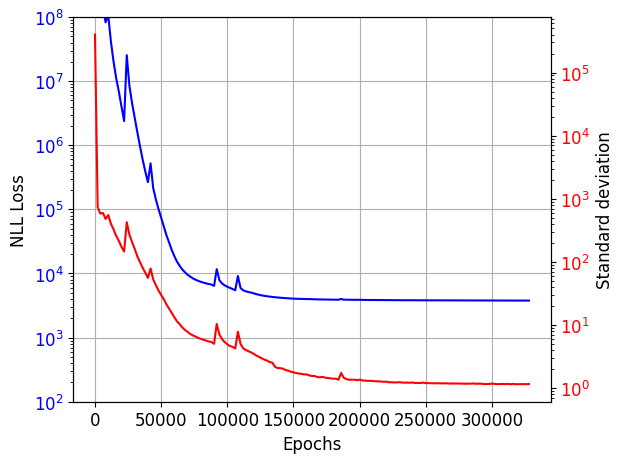
\includegraphics[width=.7\textwidth]{images/mnist_maxpooling/run_4_loss_vs_sigma.png}
\caption{Validation loss and standard deviation from Experiment 4 on the MNIST784 dataset.}
\label{fig:mnist_run_4_loss_vs_sigma}
\end{figure}